\documentclass[13pt]{article}

% Packages
\usepackage[margin= 1.5in]{geometry}
\usepackage{titlesec}
\usepackage{placeins}
\usepackage{lipsum} % For dummy text
\usepackage{graphicx} % Required for inserting images
\usepackage{booktabs}
\usepackage{siunitx}
\usepackage{caption}
\usepackage{booktabs}
\usepackage{subfig}
\usepackage{bbm}
\usepackage{amsmath, amssymb}


% Title
\title{Structural Estimation in Household Finance}
\author{Morteza Aghajanzadeh \and Najmeh Hajimirza}
\date{December 2023}


\begin{document}

\maketitle

\section{Introduction}
This project aims to estimate three parameters, time discount factor, risk aversion, and cost of stock market participation in a life cycle model of portfolio choices. In this regard, Section 2 explains the model estimation procedure and results. Section 3 presents the counterfactual analysis to examine the effect of existing capital income tax, being more risk-averse and having no cost of participation on moments estimation. Sections 4 and 5 examine model robustness and subsample heterogeneity.

\section{Model Estimation}

The individual in our model has the following optimization program:
\begin{equation*}
U = \max_{C_{iT}(\cdot), \pi_{iT}(\cdot), W_{it}} \mathbb{E} \left\{
\sum_{t=0}^{T-1} \beta^t \frac{C_{i, t}^{1-\gamma}}{1-\gamma} + \beta^T b \frac{W_{1}^{1-\gamma}}{1-\gamma}\right\}
\end{equation*}
subject to the constraint:
\begin{equation*}
W_{it+1} = \left[ W_{it} + Y_t - C_{it} - \phi_{it} \right] \left[ \pi_{it} R_t + (1 - \pi_{it}) R_f \right]
\end{equation*}
For the identification of the main parameters of the above model, we choose a set of relevant moments. We begin by considering three primary independent factors: the average wealth (\(E[W_{it}]\)), the average risky share given that it is positive (\(E[\pi_{it}|\pi_{it} > 0]\)), and the participation rate (\(E[\pi_{it} > 0]\)). It is quite straightforward to identify how these factors are affected by changes in other variables. A higher discount factor (\(\beta\)) leads to greater wealth accumulation. On the other hand, a higher degree of risk aversion (\(\gamma\)) leads to a decrease in the optimal equity share. Additionally, a higher fixed participation cost prevents households with a small optimal equity share from participating. Finally, we add the mean wealth at retirement (\(E[W_{iT}]\)) to increase the precision of the estimation. It helps to understand how households plan for retirement and engage in consumption smoothing, adjusting their savings and investment strategies over time.
\\\\
To estimate the main parameters of this model, we apply the approximate SMM method. We first define a range for parameters according to \(\beta \in [0.8, 0.99]\), \(\gamma \in [1, 5]\), and \(\Phi \in [0, 0.01]\). Then, we use the Halton sequence to generate a set of quasirandom points in a 3-dimensional space of parameters as an initial value for each of our parameters and extract the first 1000 points from the sequence as a training set. Next, we solve the individual optimization program by defining grid points for states and choices and using backward iteration on the value function. Further, we simulate the set of 7 moments for a cohort of 100,000 individuals according to the \texttt{simul.m} function provided and store it in the \texttt{Allm.mat} file.
\\\\
To generate the approximate moment function, we first create a second-order polynomial approximation of the main parameters using the \texttt{makeitpoly.m} function. Then, we fit each of the targeted moments by the GLS method based on quadratic parameters. We assign weights to individual observations in the fit model based on how close those observations are to a target moment. While the efficient choice for the weight matrix is the inverse var-cov matrix of empirical moments, we use the inverse of the sum of squared differences between simulated moments and target moments, as we do not have the variance of empirical moments. The weights are normalized by dividing each weight by the maximum weight. After fitting the model, we can compute the residuals as the difference between the selected simulated moments and their fitted values counterparts and assess the fit of the model by computing \(R^2\) to compare the variance of the residuals with the variance of the observed moments.
\begin{table}[!htbp]
    \centering
    \caption{\textbf{Assessment of the Fit of Estimated Values for Targeted Moments}\\
    \small{
    This table presents an assessment of the fit for estimated values corresponding to targeted moments in the model. The computed R-squared values indicate the proportion of variance captured in the residuals compared to the observed moments.
    }
    }
    \begin{tabular}{lcccc}
        \hline
        & $E[\pi_{it} > 0]$ & $E[\pi_{it}|\pi_{it} > 0]$ & $E[W_{it}]$ & $E[W_{iT}]$ \\
        \hline
        R-squared & 0.3714 & 0.6676 & 0.5049 & 0.9204 \\
        \hline
    \end{tabular}
    \label{tab:fit assessment}
\end{table}

\begin{table}[!htbp]
    \centering
    \caption{\textbf{Estimates of Parameters and Targeted Life Cycle Moments}\\
    \small{
    This table reports the estimated parameters in the approximate SMM estimation in panel A, and the set of targeted life cycle moments in panel B. The selected moments are participation rate, conditional mean risk, mean wealth, and mean wealth at retirement. 
    }
    }
    \begin{tabular}{lr}
        \hline
        \textbf{A. Estimated Parameters:} & \\
        Discount factor (\(\beta\)) & 0.9519 \\
        Risk aversion (\(\gamma\)) & 2.0143 \\
        Participation cost (\(\phi\)) & 0.0024 \\
        \hline
        \textbf{B. Targeted Life Cycle Moments:} & \\
        Participation Rate & \checkmark \\
        Mean Risky Share & \\
        Conditional Mean Risky & \checkmark \\
        Mean Wealth & \checkmark \\
        Std Wealth & \\
        Mean Wealth at Retirement & \checkmark \\
        Std Wealth at Retirement & \\
        \hline
    \end{tabular}
    \label{tab:estimates}
\end{table}

Now, by having the approximate moment function, we can perform an approximate SMM by executing an optimization loop (25 iterations) to minimize the approximation loss. This involves adjusting a set of parameters to refine the best parameter set that has the best alignment with the target moments.Table~\ref{tab:estimates} and Table~\ref{tab:moments} report the estimated parameters and corresponding simulated moments versus their actual counterparts, respectively. Our estimates are close to Catherine (2021), which finds \(\beta = 0.956\) and \(\phi = 0.005\). The estimation for \(\gamma\) is 2.1, which is lower than the usual estimate in structural literature; however, it is near the calibration amount in the life cycle consumption savings models.

\begin{table}[!htbp]
    \centering
    \caption{\textbf{Moment Conditions} \\ 
    \small{
    This table reports simulated versus actual moments in the approximate SMM estimation. With the exception of the final two rows, which present the mean and standard deviation of wealth at the retirement age, all other rows present statistics across all individuals and years, with observations carrying equal weight.
    }
    }
    \begin{tabular}{lccc}
        \hline
        \textbf{Moment} & \textbf{Description} & \textbf{Actual} & \textbf{Simulated} \\
        \hline
        \(E[\pi_{it} > 0]\) & Participation Rate & 0.8399 & 0.8608 \\
        \(E[\pi_{it}]\) & Mean Risky Share & 0.5941 & 0.5762 \\
        \(E[\pi_{it}|\pi_{it} > 0]\) & Conditional Mean Risky & 0.7073 & 0.6694 \\
        \(E[W_{it}]\) & Mean Wealth & 1.2151 & 1.0138 \\
        \(STD[W_{it}]\) & Std Wealth & 1.9791 & 1.7300 \\
        \(E[W_{iT}]\) & Mean Wealth at Retirement & 4.9608 & 4.8385 \\
        \(STD[W_{iT}]\) & Std Wealth at Retirement & 0.4073 & 0.3089 \\
        \hline
    \end{tabular}
    \label{tab:moments}
\end{table}
\section{Counterfactual analyses}
We now want to examine the effect of introducing a capital income tax of 30\% on our estimated moments, particularly on the mean of wealth at retirement. In this regard, our constraint becomes as follows:
\begin{equation*}
W_{it+1} = \left[ W_{it} + Y_t - C_{it} - \phi_{it} \right] \left[ \pi_{it}R_t + (1 - \pi_{it})R_f - \pi_{it}r_t\tau - (1 - \pi_{it})r_f\tau \right],
\end{equation*}
where \(\tau\) is the rate of capital tax.
\\\\
If we consider that all individuals overall period have the same pattern of investment behavior, we can calculate a present value of capital tax revenue through the following back-of-envelope calculations:
\begin{equation*}
\begin{aligned}
\text{Tax revenue} =\ & E[\pi_{it}] \cdot \sum_{t=0}^{T-1} \frac{\tau \cdot E[W_{it}] \cdot \left(E[\pi_{it}] \cdot \max(r_t, 0) + (1 - E[\pi_{it}]) \cdot \text{r}_{f}\right)}{(1 + \text{r}_{f})^t} \\
&+ \\
&\left(1 - E[\pi_{it}]\right) \cdot \sum_{t=0}^{T-1} \frac{\tau \cdot E[W_{it}] \cdot \text{r}_{f}}{(1 + \text{r}_{f})^t}
\end{aligned}
\end{equation*}
which shows the tax revenue under these assumptions will be equal to 1.0484 in the present value. 
Table~\ref{tab:counter_moments} shows the simulated moments for different versions of our model. Column (1) corresponds to the baseline model, as specified in Section II, with no capital tax (\(\tau=0\)). Column (2) presents the results from a version of the model with \(\tau=30\%\). Then, we eliminated participation cost from the model with capital income tax in column (3). Column (4) shows the results from a version of the model that has doubled the risk aversion parameter within the capital income tax policy. We changed the capital income tax model one at a time. As such, we analyze how the change of each of these parameters affects the simulated moments of our estimation.
\begin{table}[!htbp]
    \centering
    \caption{\textbf{Counterfactual moments}\\
    \small{
   This table displays the results of a series of counterfactual experiments in which we analyze the impact of introducing a capital income tax and modifying certain parameters in our model. The first column shows the simulated outcomes of our base model which does not include a capital income tax. The second column exhibits the corresponding simulated outcomes when a 30\% capital income tax is incorporated into the model. The third column demonstrates the simulated outcomes of the capital income tax model after removing the participation cost parameter. Lastly, column four portrays the simulated outcomes after doubling the risk aversion parameter in the capital income tax model.
    }
    }
    \label{tab:counter_moments}
    \begin{tabular}{lllll}
& $\tau =0$ & $\tau =30\%$ & $\tau =30\% \& \phi = 0$ & $\tau =30\% \& \gamma = 2\gamma$ \\ 
\hline 
$E[\pi_{it}>0]$ & 0.86083 & 0.69909 & 0.99999 & 0.77965 \\ 
$E[\pi_{it}]$ & 0.57623 & 0.42031 & 0.9259 & 0.36197 \\ 
$E[\pi_{it}|\pi_{it}>0]$ & 0.66938 & 0.60122 & 0.92591 & 0.46427 \\ 
$E[W_{it}]$ & 1.0138 & 0.73266 & 0.75708 & 0.39647 \\ 
$\sigma[W_{it}]$ & 1.73 & 1.4553 & 1.4602 & 1.0514 \\ 
$E[W_{iT}]$ & 4.8386 & 4.6966 & 4.7187 & 2.5541 \\ 
$\sigma[W_{iT}]$ & 0.3089 & 0.21869 & 0.21924 & 0.13271 \\ 
\hline 
\end{tabular}
\end{table}
As can be seen after introducing capital income tax, the mean of wealth at retirement decreased to 4.70 from 4.83. As capital income tax would lower the income of return on capital, it demotivates people from investing in the risky capital market, so the participation rate drops by 0.16. In column (3), we can see that excluding participation cost increases the participation rate substantially to 1, showing the vital role of this parameter on the participation of individuals in the stock market even in the presence of capital tax. Finally, in column (4), the increase of the risk aversion parameter by two times the initial value leads to lower conditional participation to 0.46 from 0.60. By comparing the change of extensive margin and intensive margin of this model, we can see the effect of an increase in risk aversion is more pronounced for the extensive margin compared to the intensive one. Also, it can be seen that a rise in the risk aversion parameter has lowered the mean wealth of all individuals over the years and that of retirement. If we consider that all individuals overall period have the same pattern of investment behavior, we can calculate a present value of capital tax revenue through the following back-of-envelope calculations:
\section{Robustness}
In this section, we will examine the robustness of our results to two different factors. 
First, we will examine the robustness of our results to the noise in one of our targeted moments, namely the mean wealth ($\mathbbm{E}[W_{it}] = 1.2151$). We will do this by drawing a random number from a normal distribution with a mean of 0 and a standard deviation of 0.1 and adding it to the mean wealth. We will then re-estimate the model using the new moments 1000 times and compare the results with the original estimates. The results are reported in Figure~\ref{fig:robustness_check}. 
For a better comparison of the results, we normalize the results by dividing them by the standard deviation of the results and subtracting the mean of the results, you can see the results in Figure~\ref{fig:robustness_standard_check}.

As you can see, for all the parameters, two standard error deviations from the moment will lead to a deviation of less than two standard errors from the estimated parameters. Therefore, we can conclude that our results are robust to the noise in the moments.

\begin{figure}[!htb]
    \centering
    \caption{\textbf{Impact of Noise on Mean Wealth Distribution} \\ 
    \small{
    The figure shows the distribution of the estimated parameters when we add a random number from a normal distribution with mean 0 and standard deviation 0.1 to the mean wealth. We re-estimate the model using the new moments for 1000 times and compare the results with the original estimates.  The green line represents the original estimates. The red line represents the estimates when we add noise to the mean wealth. The blue line represents the estimates for different values of the mean wealth. The red dashed lines represent the 5th and 95th percentiles of the distribution of the estimated parameters. The black dashed line represents the true value of the moment.
    We report the results for $\beta$ in (a), $\gamma$ in (b), and $\phi$ in (c).
    }
    }
    \label{fig:robustness_check}

    \subfloat[][Robustness Check for $\beta$]{
    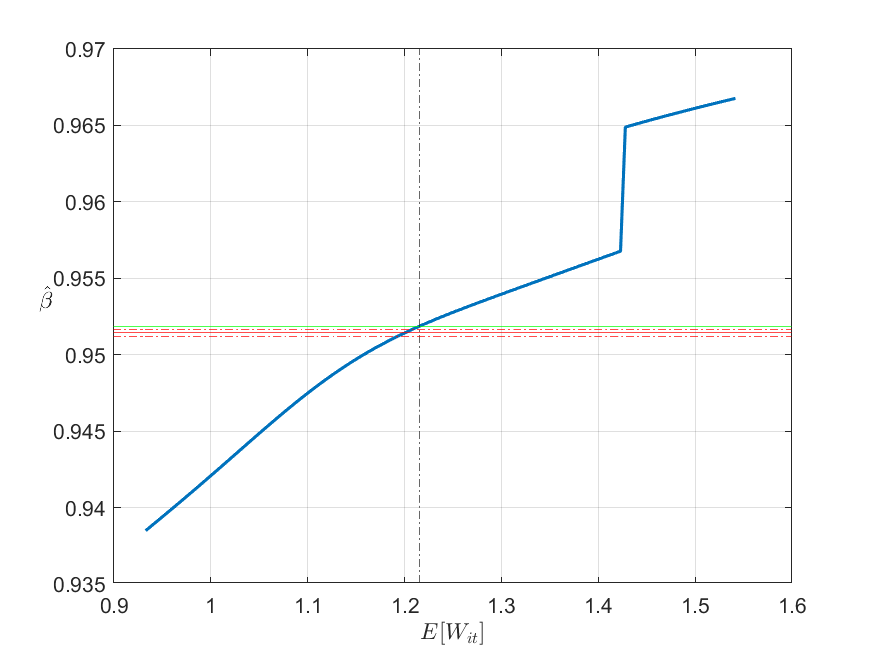
\includegraphics[width=0.45\linewidth]{Figures/robustness_check_parameterbeta.png}
    }   
    \subfloat[][Robustness Check for $\gamma$]{
    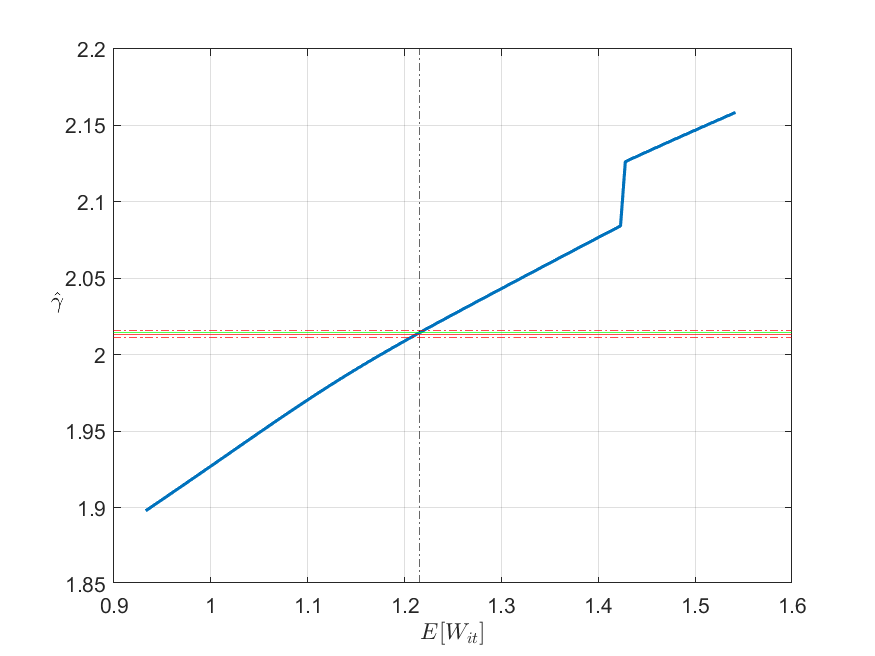
\includegraphics[width=0.45\linewidth]{Figures/robustness_check_parametergamma.png}
    }\\
    \subfloat[][Robustness Check for $\phi$]{
    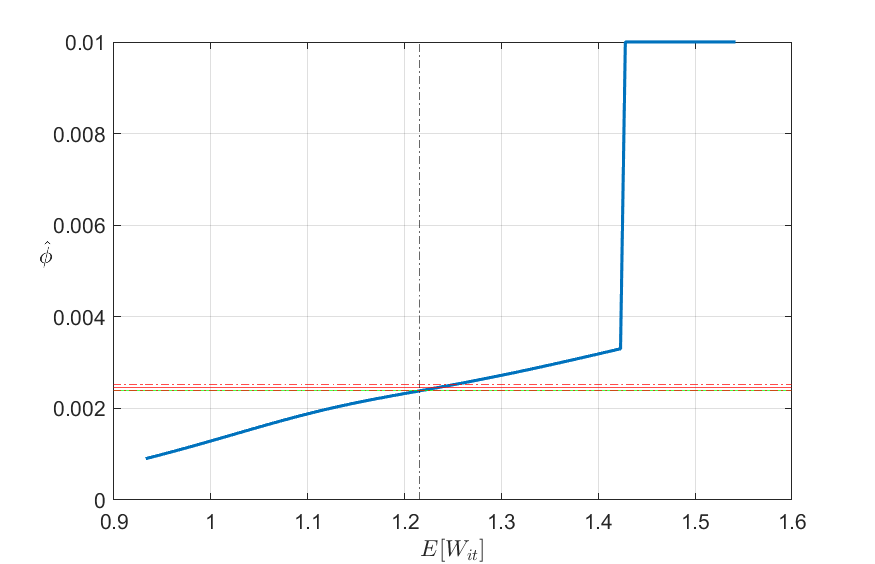
\includegraphics[width=0.45\linewidth]{Figures/robustness_check_parameterphi.png}
    }
\end{figure}
\begin{figure}[!htb]
    \centering
    \caption{\textbf{Impact of Noise on Mean Wealth Distribution (Standardize)} \\ 
    \small{
    The figure shows the distribution of the estimated parameters when we add a random number from a normal distribution with mean 0 and standard deviation 0.1 to the mean wealth. We re-estimate the model using the new moments for 1000 times and compare the results with the original estimates.  We normalize the results by dividing them by the standard deviation of the results and subtracting the mean of the results.
    The blue line represents the estimates for different values of the mean wealth. The dashed lines represent the 5th and 95th percentiles of the distribution of the estimated parameters.
    We report the results for $\beta$ in (a), $\gamma$ in (b), and $\phi$ in (c).
    }
    }
    \label{fig:robustness_standard_check}

    \subfloat[][Robustness Check for $\beta$]{
    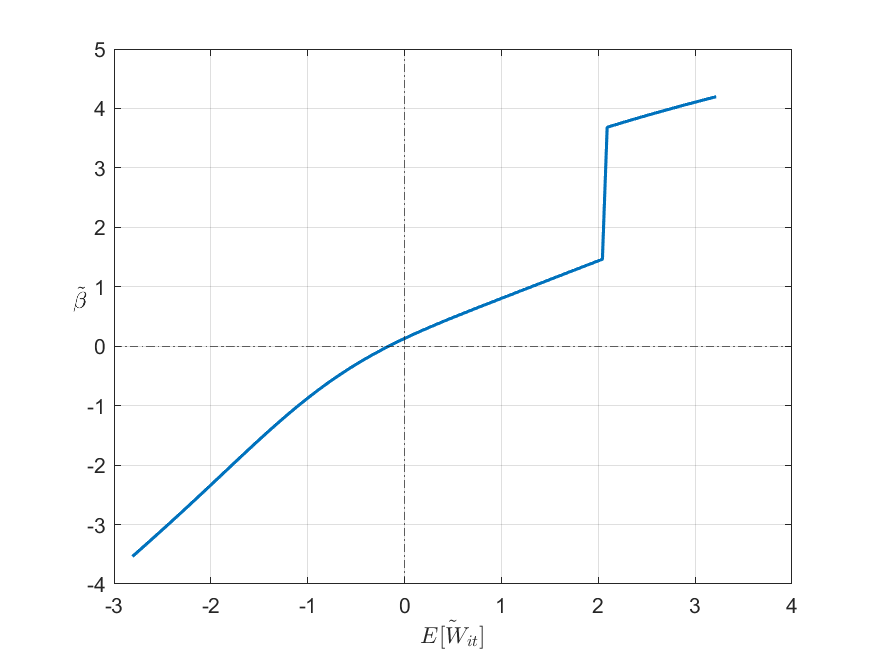
\includegraphics[width=0.45\linewidth]{Figures/robustness_check_parameter_normalize_beta.png}
    }   
    \subfloat[][Robustness Check for $\gamma$]{
    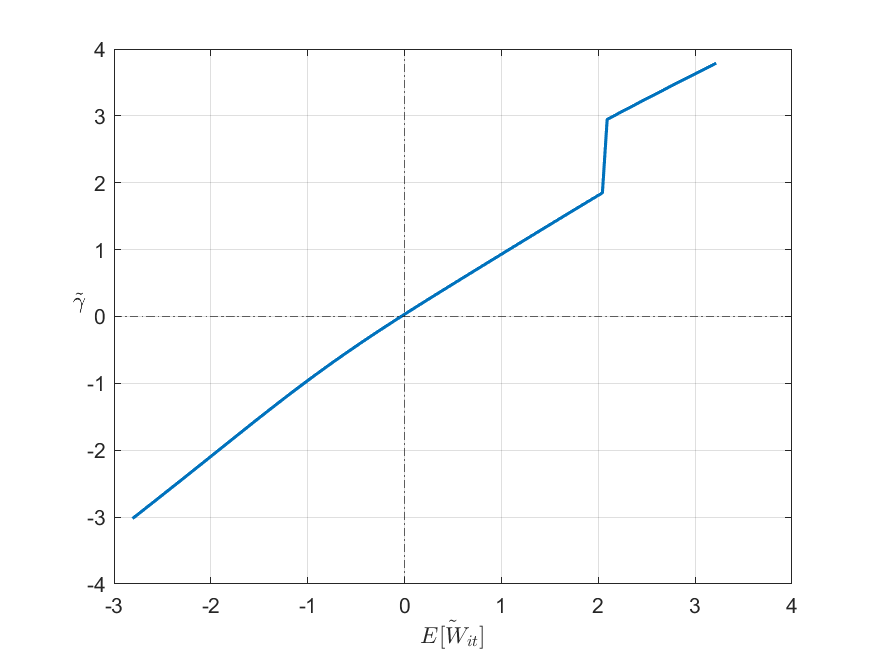
\includegraphics[width=0.45\linewidth]{Figures/robustness_check_parameter_normalize_gamma.png}
    }\\
    \subfloat[][Robustness Check for $\phi$]{
    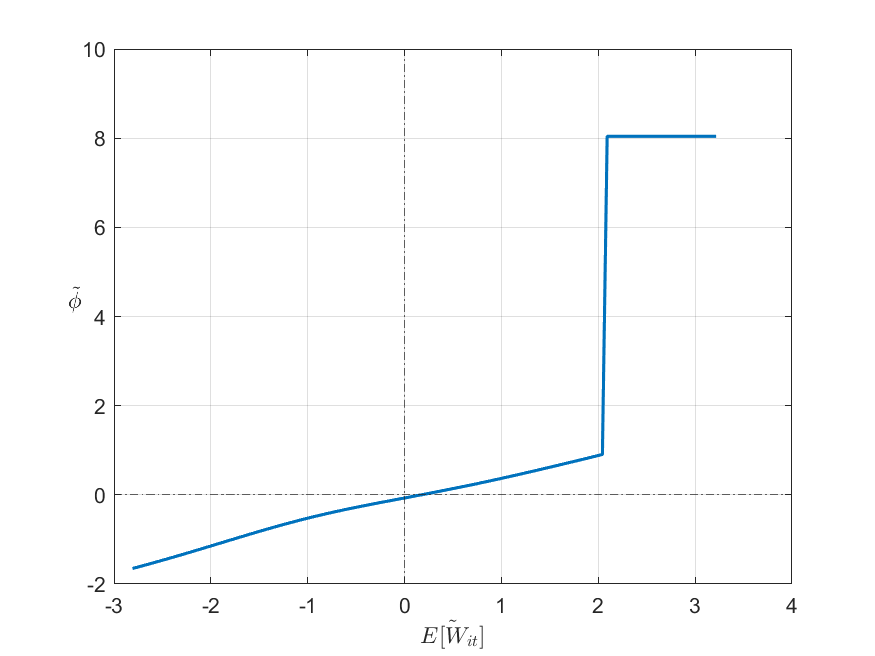
\includegraphics[width=0.45\linewidth]{Figures/robustness_check_parameter_normalize_phi.png}
    }
\end{figure}

Additionally, we will examine the robustness of our results to the inclusion of other moments in our targeted moments. We will do this by adding the mean risk share ($\mathbbm{E}[\pi_{it}] = 0.5941$), the standard deviation of wealth ($\sigma[W_{it}] = 1.9791$), and the standard deviation of wealth at retirement ($\sigma[W_{iT}] = 0.4073$) to our targeted moments. We follow the same procedure as before and add a random number from a normal distribution with a mean of 0 and a standard deviation of 0.1 to each of the moments. Furthermore, we will re-estimate the model by adding the new moments 1000 times and compare the results with the original estimates. The results are reported in Figure~\ref{fig:moment_inclusion}.

When we put in the average risky share, things stay pretty much the same in our results. But, when we add in how much wealth varies and its distribution when people retire, the results change a lot. This means that how people's wealth changes and how it's spread out when they retire are important factors that really affect the results. It shows us that some things have a bigger impact on how reliable our model is.



\begin{figure}[!htb]
    \centering
    \caption{\textbf{Impact of Introducing Noisy Moment on Parameter Estimation} \\ 
    \small{
    The figure shows estimation results when a single moment is introduced alongside the targeted moments. Specifically, we incorporate a random number from a normal distribution with a mean of 0 and a standard deviation of 0.1 to create a confidence interval, while the other targeted moments remain noise-free. We re-estimate the model using the new targeted moments for 1000 times and compare the results with the original estimates. The blue line represents the 5th and 95th percentiles of the distribution of estimated parameters, while the red line signifies the estimation results when noise is introduced only in the mean wealth. Results for $\beta$ are presented in (a), $\gamma$ in (b), and $\phi$ in (c).
    }
    }
    \label{fig:moment_inclusion}

    \subfloat[][Moment Inclusion for $\beta$]{
    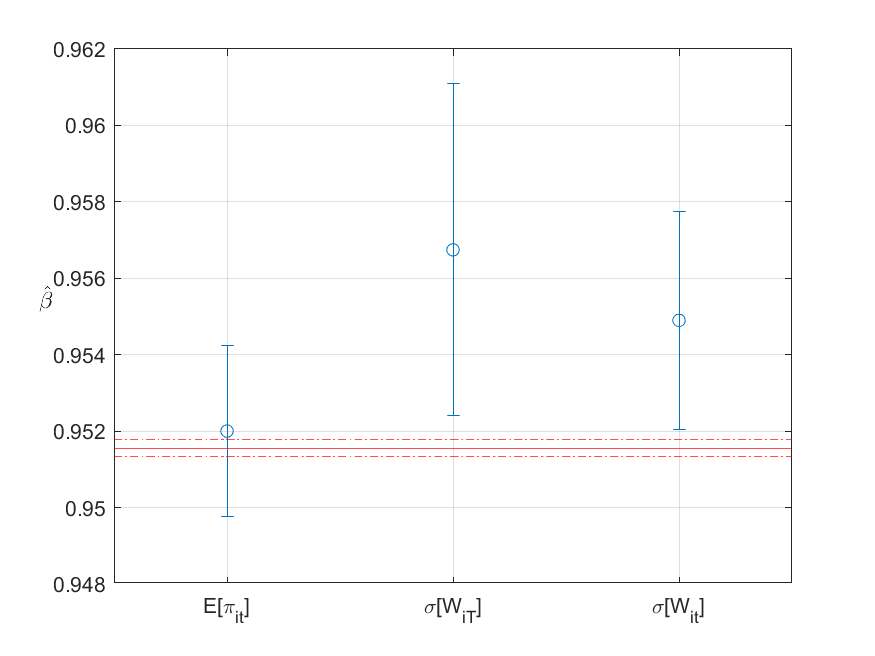
\includegraphics[width=0.45\linewidth]{Figures/moment_inclusion_check_parameterbeta.png}
    }   
    \subfloat[][Moment Inclusion for $\gamma$]{
    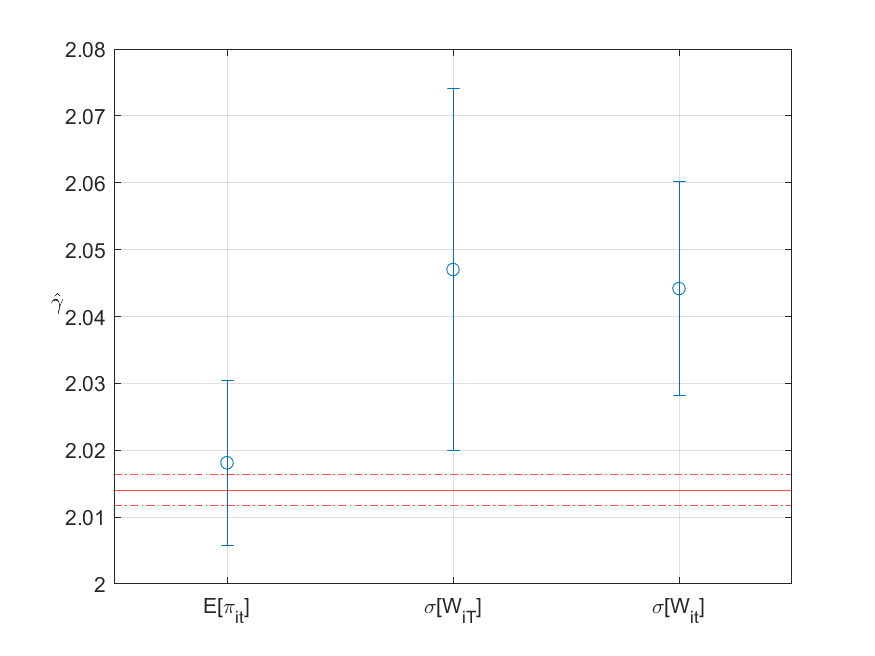
\includegraphics[width=0.45\linewidth]{Figures/moment_inclusion_check_parametergamma.png}
    }\\
    \subfloat[][Moment Inclusion for $\phi$]{
    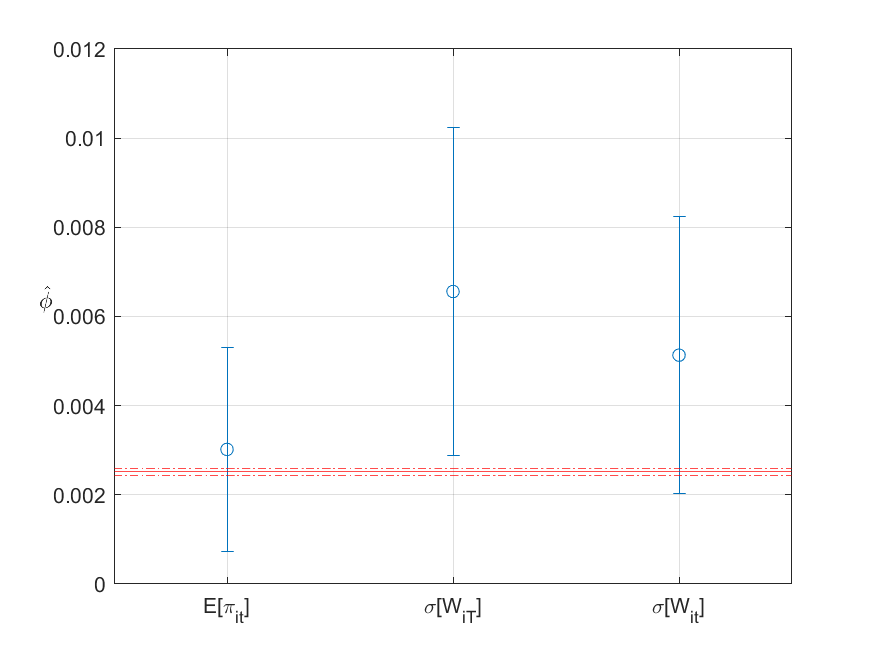
\includegraphics[width=0.45\linewidth]{Figures/moment_inclusion_check_parameterphi.png}
    }
\end{figure}

\FloatBarrier
\section{Heterogeneity}
In this section, following the instructions, we will create two sub-sample with the same population with different characteristics. You can find the characteristics of the two sub-samples in Table~\ref{tab:heterogeneity_estimation}. We will then simulate the model for each sub-sample and calculate each moment for each sub-sample. Then we can construct the moments for the whole population by taking the weighted average of the moments for each sub-sample. The results are reported in Table~\ref{tab:heterogeneity_moments}.

Now we have the new moments for the whole population, we can re-estimate the model using the new moments. The results are reported in Table~\ref{tab:heterogeneity_estimation}. As we can see, the estimated parameters are not close to the original estimates. This exercise shows that if you have a heterogeneous population, you can't just take the average of the moments and estimate the model using the average moments. You have to take into account the heterogeneity of the population and estimate the model using the moments for each sub-sample. Otherwise, you will get the wrong results. 


\begin{table}[!htbp]
    \centering
    \caption{\textbf{Heterogeneous Analysis: Characteristics and Moments Comparison} \\ 
    \small{
        This table presents findings from the analysis of heterogeneous sub-samples. Sub-table (a) details the characteristics of the main model and the two sub-samples, with the last column displaying estimated parameters derived from moments calculated using data from both sub-samples. Sub-table (b) provides information on simulated and actual moments for the main model and the two sub-samples
    }
    }

    \subfloat[][Parameters Calibration and Estimation]{
        \label{tab:heterogeneity_estimation}
    \resizebox{.85\textwidth}{!}{
    \begin{tabular}{lllll}
& Previous Estimation & Type I & Type II & Estimated Value \\ 
\hline 
$\beta$ & 0.95186 & 0.96186 & 0.94186 & 0.96525 \\ 
$\gamma$ & 2.0143 & 1.5143 & 2.5143 & 1.8431 \\ 
$\phi$ & 0.0023818 & 0 & 0.0047637 & 0.0063221 \\ 
\hline 
\end{tabular}
    } 
    }
    
    \subfloat[][Simulated Moments and Actual Moments]{
        \label{tab:heterogeneity_moments}
    \resizebox{.85\textwidth}{!}{
    \begin{tabular}{lllll}
& m & $m^I$ & $m^{II}$ & $m^*$ \\ 
\hline 
$E[\pi_{it}>0]$ & 0.86084 & 1 & 0.43405 & 0.71702 \\ 
$E[\pi_{it}]$ & 0.57623 & 1 & 0.3681 & 0.68405 \\ 
$E[\pi_{it}|\pi_{it}>0]$ & 0.66938 & 1 & 0.84807 & 0.92404 \\ 
$E[W_{it}]$ & 1.0139 & 7.1244 & 0.53859 & 3.8315 \\ 
$\sigma[W_{it}]$ & 1.7301 & 5.16 & 1.1442 & 3.1521 \\ 
$E[W_{iT}]$ & 4.8386 & 10.3688 & 3.5997 & 6.9843 \\ 
$\sigma[W_{iT}]$ & 0.30891 & 0.88554 & 0.13334 & 0.50944 \\ 
\hline 
\end{tabular}
    }
    }
\end{table}



\end{document}










